\onecolumn
\newpage

\appendices
\section{Fokusgrupper}
\subsection{Fokusgrupp 1} 

\textbf{Transkriberad ljudinspelning från Fokusgrupp 1} \\

Anna: Vad tycker ni om det allmänna utseendet av prototypen? \\

Person 5: Jag måste bara säga en sak innan vi kastar oss in i den frågan. Det beror mycket på hur mycket vetskap man har innan man använder den här sidan, det är avgörande tror jag. Jag tycker själv såhär .. Ja nu vet jag ungefär vad jag har att förvänta mig och därför har jag hög acceptansnivån för utseendet. Om det ska vara en catchy-säljigt sida då tror jag att det finns jobb att göra, det är mitt inspel på det. Vem är jag, vart kommer jag ifrån, är det någon sökning på nätet som jag har hittat hit eller svenska spel som har gjort en stor upphandling av kurser? Sånt behöver man veta innan man sätter sig in i denna rollen. För mig har det bäring på det med utseendet och sådär. Ska det vara säljigt eller bara funktionellt? Så säligt är det inte tycker jag, mer funktionellt. 

Person 2: Jag tycker att den är inbjudande för att den är enkel och det är inte jättemycket textmassor utan det är ganska instinktivt hur jag ska börja klicka. Det finns en pil där jag ska trycka, och det är ganska  intuitivt att veta när jag ska komma igång. Inte jättemycket text vilket jag tycker är bra, bilder färger. Inte så att jag blir förvirrad över var jag ska börja. Sen vet jag inte om den är speciellt inbjudande.\\

Person 1: Jag blir lite fundersam när man tittar på första sida, \enquote{learning EQ och self leadership}, det är ju lite gran den lingon som är inom ledarskaps utveckling. Man kanske kan paketera det lite grann så att det inte blir så internt coach perspektiv. För jag gillar att ha slutprodukten synlig, som något slags kontrakt. Sen kan man fundera på vad man kan göra med den för att befästa den. Oavsett om du har kommit in i den här processen inom att vara i en mobil värld eller i en fysisk dialog så har man ungefär skapat samma kontrakt. Den som är tricket här är att få det levande över en tid och då måste du kanske befästa detta kontraktet på något sätt, kanske att man distribuerar det eller att du får möteskallelser automatiskt in i telefonen för att faktiskt göra dessa aktions som du kommit överens. \\

Person 5: Det är bra  med kort information, instruktion, inga sådana här tio minuters lyssningar. \\

Person 2: Ja det var verkligen lagom långt klipp. Jag tänkte på när man klickar in där så hamnar man mitt inne i två av tio lektioner. Då är det bra att det finns en tidslinje, så man ser hur långt den är. Jag skulle nog ha en annan förstasida oavsett vart den landar.\\

Person 1: Jag gillade det personliga tilltalet i videon. Sen kan man fundera på om man i processen kan få ännu mer personligare. I början är det okej att det är generellt, utan någon personlig information. För just videon signalerar ju någon form utav personlig dialog. Men om det bara är en allmän instruktion som är lika oavsett vad jag svara i olika steg så är den kanske lite besviken på den. \\

Person 5: Jag gillar att det var funktionellt, här ska man trycka, man har inte så mycket andra initiativ eller möjligheter. Inte så mycket ”buzz”. Det är funktion snarare än att det är feeling. Det är inte så säljande, inte så wowigt, inte så mycket konfetti, utan det är funktion.. tryck här och sedan gå vidare. Det behöver inte vara fel men det är min känsla. \\ 

Anna: Är det lätt att förstå vad du ska göra som användare? hur många gånger ska jag göra de här övningarna? \\

Hela gruppen: Ja\\

Person 2: Se så ser man inte pilen förrän man trycker på skärmen, utan man ser bara en bild, då tycker man -har man fastnat nu eller. \\

Person 5: Jag tycker det är självklart när man markerar, här på MAC datorn, det man vill klicka på så blir det ett förstoringsglas. Det var inte glasklart vart man ska markera, för det fanns ingen punkt eller checkbox, ska jag klicka på texten här eller.. Det var inte super tydligt. \\

Person 2: Sen kan man ju tänka sig att ser man dåligt så är det lite för grått, texten är för grå. Så jag får ju då använda förstoringsglas \\

Person 5: Kan man göra en sådan här grej att vid markeringen där när man hovrar över texten så går fonten upp. Bara så att man ser \\

Person 4: Är inte det super irriterande? \\

Person 5: Bara för att markera, \enquote{här är du} liksom. \\

Person 4: MAC:en har ju en docka här nere med applikationer och sedan så ett förstoringsglas, det är det första man stänger av så den inte håller på att förstora och förminska. Men det är ju en annan liknelse. \\

Anna: Men var det lätt för dig att förstå vad som var nästkommande steg?\\

Person 4: Nej jag tycker inte det, det var oklart. Det första jag funderar över som förmodligen förklaras någonstans, är varför lifeintentions är viktigt. Det förklarades inte tyckte jag. Sen så är det då när man svarar och gå vidare,Men det var ju enkelt i form av att jag inte kunde gör något annat mer än att gå vidare. Inte min effort i form av okej nu har jag gjort detta, vad kommer sendan? \\

Anna: Skulle du känna att du skulle vilja se det, hur många steg du vill göra i övningen? \\

Person 4: Nu är det väldigt påverkad av hur vi tänker kring UX design på klarna, och det är solklart att det alltid ska vara så. Jag vill alltid tänka att \enquote{vad är minimal effort för att gå vidare från detta}? \\

Person 5: ja det är bra att se hur lång resan är. \\

Person 1: det var ju någon form utav en progressiv indikator, när man svarade på dessa flervalsfrågorna, det var ju bra! Men det fanns ingen övergripande på dessa tre minuterna, det saknades ju helt. Det var på enskilda moment fanns det ju så att man kunde gissa sig fram på hur lång det var men inte helheten. \\

Person 3: men ja tkr också total sammanställningen är viktig. \\

Anna: Känns appen trovärdig?\\

Person 4: om jag får gå tillbaka till detta med attraktivitet så tycker jag att attraktivitet inte viktig för seriositeten, om detta hade varit min första interaktion med appen så ser den inte seriös ut, utifrån vad man är van vid och hur saker och ting ser ut designmässigt. 
Det finns en app, som man kan klassa som en konkurrent, där man går igenom appen och går igenom sina grundvärderingar utifrån forskning så är det ett väldigt stort antal värderingar. Det tar mer effort, så jag värderar att resultatet mer i och med att det tar mer effort, så ju snabbare det går, desto mindre seriös och med som pop-quiz på Facebook. Appen ser extremt proffsig ut i jämförelse med prototypen. Men också sättet man sortera ut känns mer seriöst när det finns mer val, och jobbigare. Och problemet, när vi har testat ai-coachning, är hur människor fungerar. Hjärnan fungerar som sådan att 40 procent när vi gör saker går på autopilot, det betyder att vi använder oss av gamla vanor, dessa vanor skyddar oss från att testa nya saker. När något är för enkelt är det lättare att gå in i autopilot, gå in i en gamification snarare än att jag faktiskt reflekterar på riktigt. Och det är det svåra med sådana här typer av trainable app. \\

Anna: Hur modern kändes denna prototypen?\\

Person 4: inte alls, för att finns ingenting nytt i den, sättet att lära ut på , nä de är jättemånga som gör det, samma sak med video. Jag vet inte vad som skulle vara nytt över huvud taget.\\

Anna: Men kändes den stimulerande att använda?\\

Person 4: Jag tror att för mig, som har testat jättemånga sådana appar och försökt implementera det, det börjar inte med appen, det börjar i en annan ända, vad har hänt innan appen? Vi säger om allt annat har fungerat så är appen inte viktig, jag skulle lägga mer krut på vad som är utanför appen snarare än vad som är inuti.\\ 

Person 3: Jag tänker att det är en bra förlängning då, att man har detta som ett komplement till nästa steg. Utifrån hur Amazing Leaders jobbar här och nu så tror jag att det kan vara ett bra stöd, som en brygga in och för att få kontinuitet. \\

Person 5: Ja, för att föra folk framåt, utan att varje gång behöva träffas. Mekanism för att driva utvecklingen för individerna framåt. Om vi har haft ett möte med, säg Ursula nu då, så har vi dessa tre aktiviteter och övningar som vi har på papper och som vi kan följa upp.\\ 

Person 1: Jag är inne på samma sak, man behöver nästan bestämma sig, antingen så är det förberedande och då är det inte seriositet så viktigt, då är det mer ett insamlingsmoment. Skriv ned dessa 10 saker i din bok, de där har man ju väldigt svårt att ta sig för. Detta skulle kunna vara ett enkelt sätt för att jag inte ska behöva gå tillbaka till mina anteckningar. Den andra biten som jag tror kan va intressant också är den här resultat effekten, nån action därefter. vi säger det här kontraktet du har gjort i nån form utav fysiks dialog, dokumentationen och exekveringen utav det långsiktiga är något man kan bocka av. Lite som gamificaition, jag har gjort detta, det som vi kom överens om. \\

\subsection{Fokusgrupp 2}

\textbf{Transkriberad ljudinspelning från Fokusgrupp 1}
\\

Anna: Vad tycker ni om det allmänna utseendet av prototypen? \\

Person 1: Jag gillade det på första sidan, detta med att det ser ut som en scroll. Så att man kan se progressen. Vill alltid ha kontroll på hur långt jag kommit, så det är bra. Vill veta vart är jag, hur mycket har jag kvar, är det lönt att börja på en ny osv. \\

Person 4: Det är nästan så man skulle vilja se vilket kapitel och hur lång övningen är, så man förstår vad man ger sig in på. \\

Person 1: Men bara som någon slags förstaupplevelse, vart är jag för någonstans? \\

Var prototypen inbjudande?\\

Person 3: ja det tycker jag. Det var tydligt och rent, det var lätt att komma igång med det. Lättillgängligt. \\

Person 2: Jag är oftast väldigt rastlös när man tittar i en telefon, vill se direkt vad det är, inte så mycket text utan det ska vara tydligt och enkelt. Förstår direkt vad det är man gör. \\

Person 1: Ja precis, lite det här med att less is more. Få grejer men man ska direkt förstå vad som ska göras. \\

Person 3: Det var lagom långa filmer, så fort dom blir för långa så tappar jag uppmärksamheten. \\

Person 3: Gå framåt och bakåt saknade jag \\

Person 1: Första sidan var bra, men att man får mer kontroll. Man såg att det var en film men det gick inte se hur lång den var, men jag vill veta hur lång den är. Om det är andra gången jag går in så vill jag dra fram 45 sekunder om jag redan har sett på det. \\

Hur tydlig var prototypen? \\

Person 3: Man kände att det var en prototyp, just för att dessa småsaker var inte mer. Blir mer nyfiken på hur nästa version kommer att vara \\

Person 1: Sådär, för att den känns lite buggig. \\

Person 4: det var inte riktigt tydligt hur man skulle klicka klart tycker jag. Lite mer intuitivt \\

Vad det lätt att förstå vad som förväntades? \\

Person 3: Man förstod att det var en film man skulle kolla på i och med att det var en playknapp. Inte svårt att förstå men jag fick inte sammanhanget. The why, varför göra detta, om jag får reda på det så kör jag vidare sedan utan att tänka.\\

Person 4: Inte riktigt tydlig kontext. \\

Förstod man vad som var nästkommande steg?\\

Person 1: ja men det tycker jag, man tog ju sig framåt för att det inte fanns så många andra alternativ. \\

Person 3: Jag gillade att det var lika dana blåa bars. Den blå knappformen hjälpte tydligheten. Man fattade att det var en form av action. \\ 

Hur pålitlig kändes prototypen?\\

Person 2: Det blir nog en utmaning att få till det i en kort video. Annars kommer man ju inte orka med att kolla. Hitta så att det blir seriös med inte för lång \\

Person 1: Tex videon, den skulle behöva vara studioproducerad, känns lite ihopkok med telefonfilmen, det tappar trovärdighet. Alla detaljer behöver ha vass kvalité för att kännas trovärdig \\

Hur modern kändes prototypen? \\

Person 3: Sådär, det finns ju mycket sånt men den kändes trevlig, mer trevlig än nytänkande typ. \\ 

Person 2: Ja precis, jag håller med.\\

Person 1: Gillar första sidan, den var fräsch. \\

Person 3: Den här blir mer personlig än om det bara skulle vara grafiskt. \\

Kändes den stimulerande? \\

Person 1:  Jag gillade att  interaktivitet i den, och att det var interaktivitet som var personlig för mig. Det tror jag är nyckeln, att det inte är generellt för alla, göra något och reflektera är viktigt. \\

Person 3: Skulle nog vilja att det fanns en fördjupningsknapp om man ex skulle vilja läsa mer om vad EQ var, vad menas med vad som var mina actions. Då får man ännu en nivå på det \\

\subsection{Fokusgrupp 3}

\textbf{Transkriberad ljudinspelning från Fokusgrupp 3} \\

Person 1: I liked that it had clear intentions, very specific for the person who uses it. And a clear flow of the prototype. But I would like an option to skip the videos and have a text or something. \\

Person 3: I think it looked really nice, but I think its a bit hard to understand whats the mission is. And I think that if you could show it in a graphical way before she start to tak, other wise its hard to get the point.  But I think it’s nice to have someone talking for once, because usually it’s a lot of text and so.\\

Person 4:  I agree with both of you,  and the interface Is okay.  In the whole scope it’s good. But I would like to have a functionality to go back and maybe repeat, if you come up with something more that you would write for your answer. \\

Person 5 : I really liked the person person who talked, she was calm.  The flow is structured well. \\

Person 3: Another thing; maybe it should visualize the total journey, like, I’m here right now, I started there and this is the end.  It’s very important to understand the mission, the goal and why, how , what and where I am right now. \\

Person 1: Yes, you want to se progress of what you are doing. But you don’t have to be forced to do it , if you want to see your progress you can do it. \\

Person 5: Maybe it can be a bar that you could hide if you don’t want to see the progress. \\ 

Person 2: I liked the design, I think that colors is nice, easy with the flow. I understand what to do. Then I agree on the alternative to the video, maybe show a text , if you don’t able to have sound. And a progress bar Is nice to see where you have started and were you going, so you could orient yourself a bit were you are. \\

Person 3: I think that it was not that clear, you have to be more clear in the beginning of what the goals for this exercise is. What is the goal and mission.  Why are you starting here? What is the steps? And I think it’s important to visualize it. \\ 

Person 1: The app is clear, but If I have a goal how would I know that the app is helping me reach that goal? When I’m in the app and chosen my intentions, that is clear my question is that, does it help me in any way? \\

Person 3: its not clear what the purpose is and if the app helps me. \\ 

Person 2: I think that Ursulas tone is quite serious and she framför a serious message, but the prototype itself is not that serious, it’s a bit playful.  Because of the colors, it feels like a quiz which may not seem the most serious. \\

Person 5: I think it was serious, because of the message she gave. It was reliable, didn’t think that I was playing. \\ 

Person 2: Det var inte som ett spel för mig.  Jag saknade någon slags tydlig ram,  färgmässigt, lite stringent. Den känns lite ”fladdrig”. Det är viktigt att färgtemat följer en röd tråd och är sammanhängande. Behövs lite mer tydligt att det finns en huvudmeny, om man vill backa eller om man vill pausa.  Det är svårt att svara på frågan om den är pålitlig då prototypen buggade, fick en känsla av att den lite var pålitlig då.  Fungerar inte tekniken så hoppar jag över det, det är jätteviktigt för mig. Det hade varit bra om man fick skriva noteringar eller frågor som jag har till min coach, antingen separat eller kopplat till mitt coachingpnogram. \\

Person 1: What she said about the color scheme, you can mix playfulness and seriousness but if you have a lot of colors it don’t appear so serious.  But if you have one color and have that color along the journey it changes the user experience in a positive way and upper more serious. \\

Person 3: I’ts not fun, but must it be fun? I’m not certain that it should be fun actually.  This is something for me and my journey, mor of an stimulation in that context. \\

Person 3: Stimulation for me is something that I can use in my daily life or at home. For me its a good thing if I can see that I have a benefit from it. \\

Person 3: The app should support growth so it does not have to be fun, maybe it should not be fun, then it won’t be serious. It should tot boring but not like a game either. \\

Person 4:  Personally I would only like to have that once, or else I just cancel the message or don’t read it. \\

Person 2: The fact that we know that she is an experienced coach it makes the app more reliable. But if you don’t know that she can say it in the beginning of the video. \\
\section{Enkätundersökning}

    
 \begin{figure} [H]
   \centering
   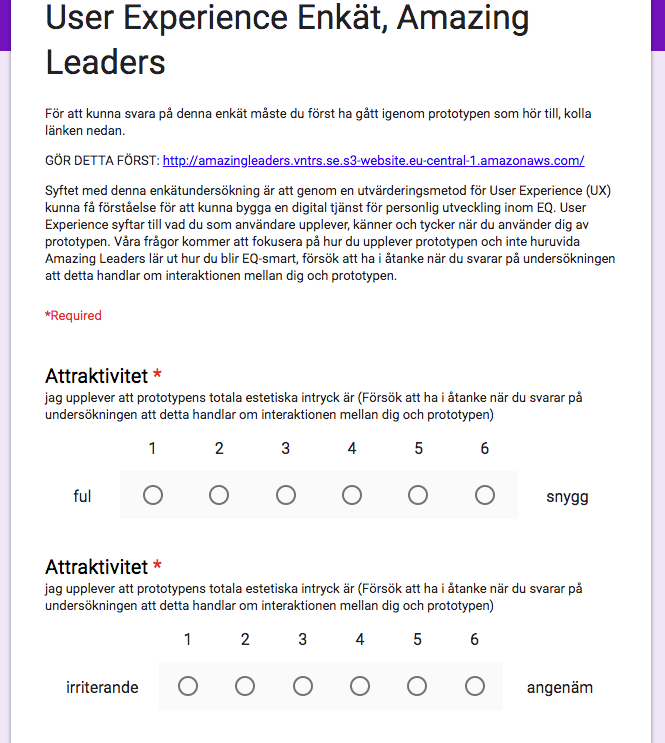
\includegraphics[scale=0.75]{form1.png}
  \captionsetup{justification=centering,margin=2cm}
  \caption{Enkätundersökning}
 \end{figure} 
 
  \begin{figure} [H]
   \centering
   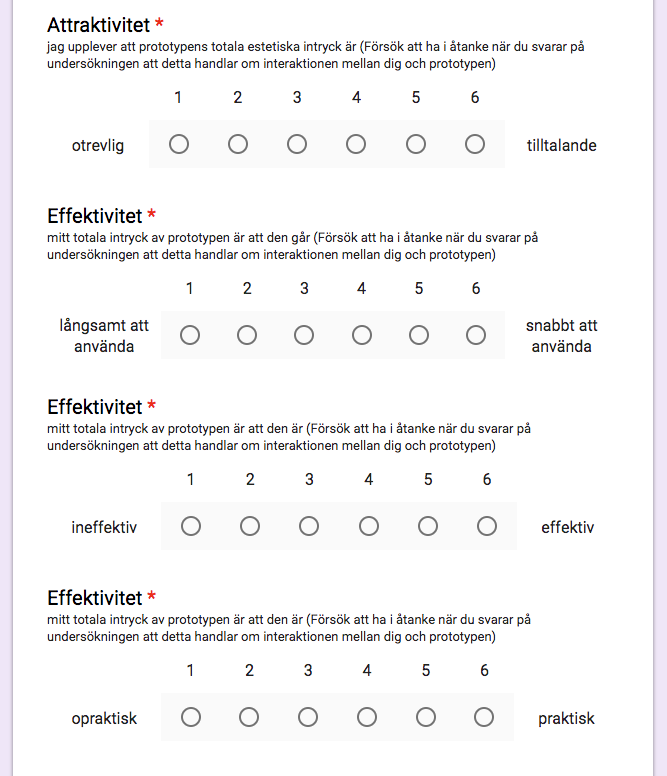
\includegraphics[scale=0.75]{form2.png}
  \captionsetup{justification=centering,margin=2cm}
  \caption{Enkätundersökning}
 \end{figure} 

 \begin{figure} [H]
   \centering
   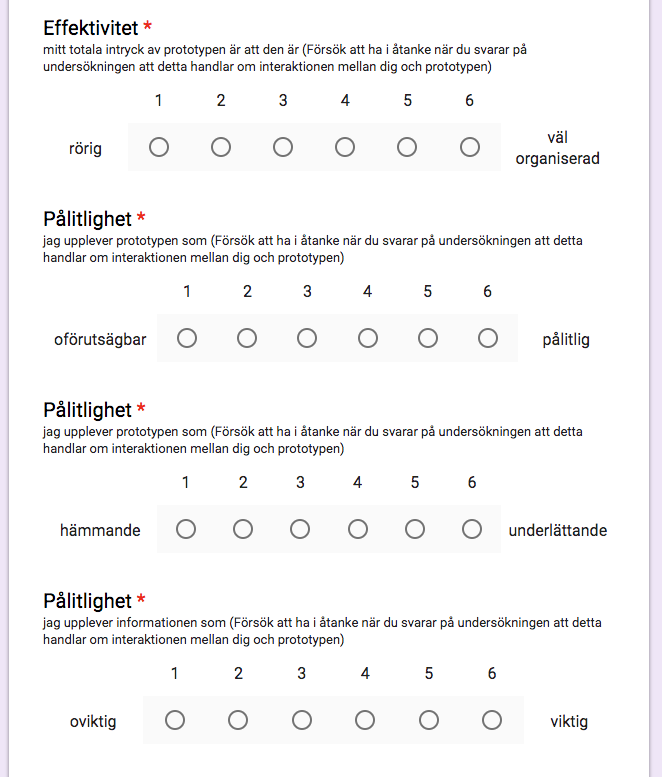
\includegraphics[scale=0.75]{form3.png}
  \captionsetup{justification=centering,margin=2cm}
  \caption{Enkätundersökning}
 \end{figure} 
 
  \begin{figure} [H]
   \centering
   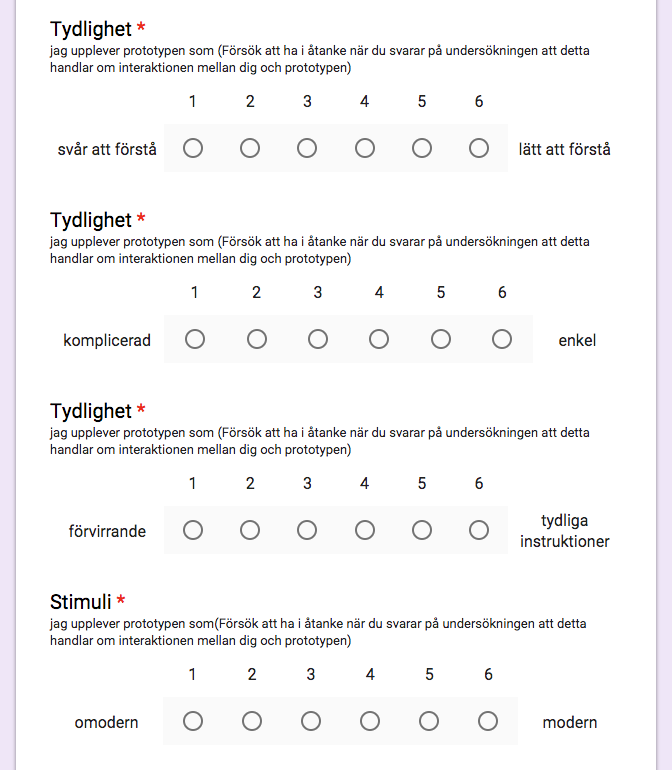
\includegraphics[scale=0.75]{form4.png}
  \captionsetup{justification=centering,margin=2cm}
  \caption{Enkätundersökning}
 \end{figure} 
 
  \begin{figure} [H]
   \centering
   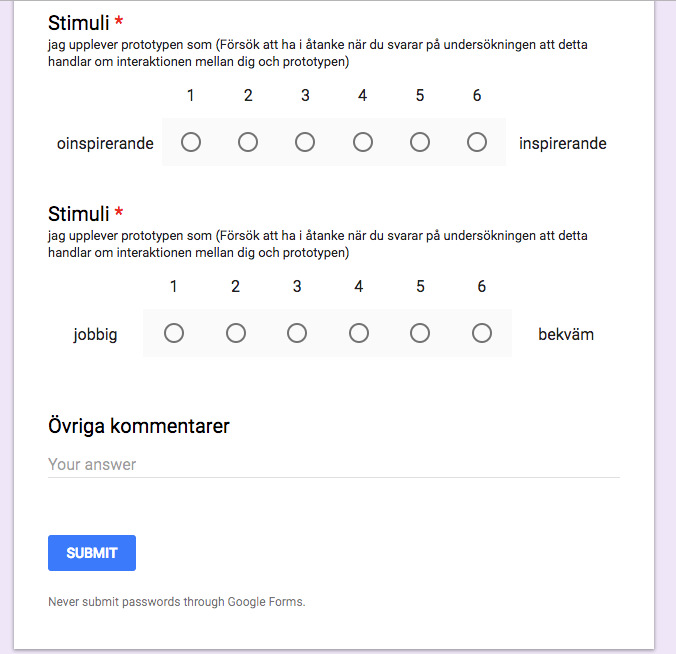
\includegraphics[scale=0.75]{form5.png}
  \captionsetup{justification=centering,margin=2cm}
  \caption{Enkätundersökning}
 \end{figure} 
